\documentclass{../UTNetLab}

\title{A Single Segment Network}
\begin{document}
\part{Network Interface Exercises}
    The following exercises use the single segment network topology shown in Fig. 1.3.
    \begin{center}
        \begin{minipage}{0.48\textwidth}
            \begin{flushleft}
                \begin{table}[H]
                    \caption{\textit{Table 1.2} The IP addresses of the hosts}
                    \centering
                    \begin{tabular}{ c c c }
                        \hline \hline
                        Host & IP Address & Subnet Mask \\
                        \hline 
                        h0 & 128.238.66.100 & 255.255.255.0 \\
                        h1 & 128.238.66.101 & 255.255.255.0 \\
                        h2 & 128.238.66.102 & 255.255.255.0 \\
                        h3 & 128.238.66.103 & 255.255.255.0 \\
                        h4 & 128.238.66.104 & 255.255.255.0 \\
                        h5 & 128.238.66.105 & 255.255.255.0 \\
                        h6 & 128.238.66.106 & 255.255.255.0 \\
                        h7 & 128.238.66.107 & 255.255.255.0 \\
                        \hline \hline
                        \end{tabular}
                \end{table}
            \end{flushleft}
        \end{minipage}
        \begin{minipage}{0.48\textwidth}
            \begin{flushright}
                \begin{figure}[H]
                    \centering
                    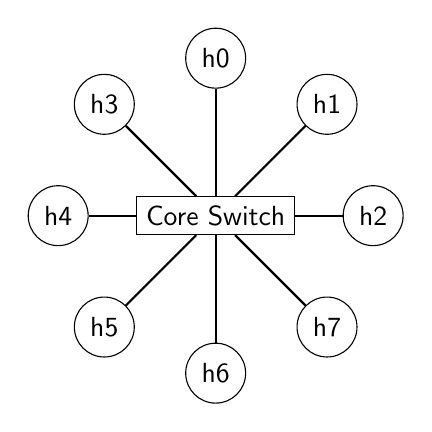
\begin{tikzpicture}[font=\sf]
                        \node[draw] (s) at (0,0){Core Switch};
                        \node[draw,circle] (h0) at (0,2){h0};
                        \node[draw,circle] (h1) at ({sqrt(2)},{sqrt(2)}){h1};
                        \node[draw,circle] (h2) at (2,0){h2};
                        \node[draw,circle] (h3) at (-{sqrt(2)},{sqrt(2)}){h3};
                        \node[draw,circle] (h4) at (-2,0){h4};
                        \node[draw,circle] (h5) at (-{sqrt(2)},-{sqrt(2)}){h5};
                        \node[draw,circle] (h6) at (0,-2){h6};
                        \node[draw,circle] (h7) at ({sqrt(2)},-{sqrt(2)}){h7};
                    
                        \draw[thick] (h0) -- (s);
                        \draw[thick] (h1) -- (s);
                        \draw[thick] (h2) -- (s);
                        \draw[thick] (h3) -- (s);
                        \draw[thick] (h4) -- (s);
                        \draw[thick] (h5) -- (s);
                        \draw[thick] (h6) -- (s);
                        \draw[thick] (h7) -- (s);
                    \end{tikzpicture}
                    \caption{\textit{Figure 1.3} A single segment network}        
                \end{figure}
            \end{flushright}
        \end{minipage}
    \end{center}

\section{Network Interfaces}
    Use the \lstinline{ifconfig -a} command to display information about the network interfaces on your host.
    Find the IP address and the net mask of your machine.
    
    \begin{report}
    \item How many interfaces does the host have?
    List all the interfaces found, give their names, and explain their functions briefly.

    \item What are the MTUs of the interfaces on your host?

    \item Is network subnetted?
    What is the reasoning for your answer? What the experimental are the reasons for subnetting?
    \end{report}


\section{Local Host Dump}
    While \lstinline[emph={your-host}]{tcpdump host your-host} is running in one command window, run \lstinline{ping 127.0.0.1} from another command window.
    
    \begin{report}
    \item From the \lstinline{ping} output, is the 127.0.0.1 interface on?
    Can you see any ICMP message sent from your host in the \lstinline{tcpdump} output?
    Why?
    \end{report}


\section{Network Statistics}
    By using \lstinline{netstat -ie}\footnote{You can use \lstinline{ifconfig} instead.} command, collect the statistics from all the hosts on the network.
    Since we use the same login name and password, we can \lstinline{telnet} to other workstations and run \lstinline{netstat -ie} there.\footnote{%
    After you are done with a remote host, you should exit the \lstinline{telnet} session before you \lstinline{telnet} to another remote host.
    Recursive \lstinline{telnet} will generate unnecessary data in the \lstinline{tcpdump} output and cause confusion.
    }

    Save the \lstinline{netstat -ie} outputs.

    If you don’t see a significant amount of output packets in the \lstinline{netstat} output, the machine was probably restarted recently. You may do this experiment later, or use the following \lstinline{socket} command to generate some network traffic:
    \begin{lstlisting}[emph={remote-host}]
socket -u -i -n200 remote-host echo
    \end{lstlisting}
    
    \begin{report}
    \item Calculate the average collision rate over all the hosts for the set of statistics you collected in this exercise.
    \end{report}

\part{ARP Exercises}
    In the following experiment, we shall examine the host ARP table and the ARP operation, including two interesting cases: proxy ARP and gratuitous ARP. You may need to ask the lab instructor for the MAC addresses of the host and router interfaces, and record these MAC addresses in Table A.1 and Table A.2 in the appendix.
    You need these MAC addresses for the exercises and lab report.

\section{ARP Table}
    Use \lstinline{arp -a} to see the entire ARP table.
    Observe that all the IP addresses displayed are on the same subnet.

    If you find that all the remote hosts are in your host’s ARP table, you need to delete a remote host (not your workstation) from the table, using:
    \footnote{If you deleted your workstation’s IP address from the ARP table by mistake, you must add the entry back in the table. See the \lstinline{arp} manual page to add.
    Note that, in order for your workstation to reply to the ARP requests, the ARP entry of your workstation must have the \lstinline{P} flag in the ARP table.}
    \begin{lstlisting}[emph={remote-host}]
arp -d remote-host
    \end{lstlisting}

    Save the ARP table for your lab report.

    While \lstinline{tcpdump -en}\footnote{You can add \lstinline{-x} flag to see hex dump.} is running, \lstinline{ping} a remote host that has no entry in your host ARP table.
    Then terminate the \lstinline{tcpdump} program.

    You can run \lstinline{wireshark &} to capture network.

    Observe the first few lines of the packet trace to see how ARP is used to resolve an IP address.

    Run \lstinline{arp -a} to see a new line added in your host’s ARP table.
    Save the new ARP table for your lab report.

    Mark the ARP request packet and the ARP reply packet in the \lstinline{wireshark} window.
    Then go to menu \textit{File/Print\ldots} to print the marked packets for your lab report (See Exercise 6 of Chapter 1).

    \begin{report}
    \item From the saved \lstinline{tcpdump} output, explain how ARP operates.
    Draw the format of a captured, ARP request and reply including each field and the value.
    \end{report}

    Your report should include the answers for the following questions.
    \begin{itemize}
        \item What is the target IP address in the ARP request?
        \item At the MAC layer, what is the destination Ethernet address of the frame carrying the ARP request?
        \item What is the \texttt{frame} type field in the Ethernet frame?
        \item Who sends the ARP reply?
    \end{itemize}

\section{ARP Timeout}
    While \lstinline[emph={your-host}]{tcpdump host your-host} is running to capture traffic from your machine, execute \lstinline{telnet 128.238.66.200}.
    Note there is no host with this IP address in the current configuration of the lab network.

    Save the \lstinline{tcpdump} output of the first few packets for the lab report.

    After getting the necessary output, terminate the \lstinline{telnet} session.

    \begin{report}
    \item From the saved \lstinline{tcpdump} output, describe how the ARP timeout and retransmission were performed.
    How many attemps were made to resolve a non-existing IP address?
    \end{report}

\section{ARP Proxy}
    The network topology for this proxy ARP exercise is shown in Fig. 2.9. We will divide the group into two subnets interconnected by a router. The IP addresses and network masks for the hosts are also given in Fig. 2.9. Change the IP address and network mask of your host accordingly (see Section 2.3.2). The IP addresses and network masks of the \textit{Router4} interfaces are the same as their default settings.
    Note that the network mask of the hosts in the 128.238.65.0 network is 255.255.0.0.

    Set IP of each network by running the following command in the hosts:
    \begin{enumerate}
        \item \lstinline[emph={x.x.x.x}]{ifconfig eth0 x.x.x.x/mask}
        \item \lstinline[emph={x.x.x.x}]{route add default gw x.x.x.x}
    \end{enumerate}
    Next we will enable the proxy ARP function on the ethernet1 interface of \textit{Router4}.
    \begin{enumerate}
        \item \lstinline{telnet} to \textit{Router4}. (Use \lstinline{telnet 128.238.64.4}, or right click on the Router and open console on GNS3.)
        \item Log in to the router, type \lstinline[language={cisco}]{enable} to enter the \textit{Privileged EXEC} mode.\footnote{We will discuss bridge and router configuration in Chapter~3.}
        \item Enter the \textit{Global Configuration} mode by typing \lstinline[language={cisco}]{config term}.
        \item Then type the following lines for each interfaces:
        \begin{itemize}
            \item \lstinline[language={cisco}]{interface f0/0 # f0/1 for another}\footnote{The name of the router interfaces may be different for various routers.
            You can find the names by typing \lstinline[language={cisco}]{write term} in the \textit{Privilege EXEC} mode.}
            \item \lstinline[language={cisco}]{ip addr x.x.x.x 255.255.255.0}
            \item \lstinline[language={cisco}]{no shut}
            \item \lstinline[language={cisco}]{ip proxy-arp}
            \item \texttt{Ctrl-Z}
            \item \lstinline[language={cisco}]{wr}
        \end{itemize}
        % \item Type \lstinline[language={cisco}]{exit} to terminate the \lstinline{telnet} session.
    \end{enumerate}
    
    Now \textit{Router4}’s \textit{ethernet1} interface can perform proxy ARP for the hosts in the 128.238.64.0 subnet.

    Run \lstinline{tcpdump -enx} on all the hosts.

    Then let the hosts in the 128.238.65.0 subnet send UDP datagrams to the hosts in the 128.238.64.0 subnet.
    For example, on \textit{h7} type:
    \begin{lstlisting}[emph={host-in-64-0-subnet}]
socket -i -u -n1 -w1000 host-in-64-0-subnet echo
    \end{lstlisting}

    When you are done with all the hosts in the 128.238.64.0 subnet, save the tcpdump output for the lab report.

    Run \lstinline{arp -a} to display the new ARP table in your host.
    Save the ARP table for your lab report.

    After the lab instructor restores the network into a single subnet (see Fig. 1.3), change the IP address and network mask of your host’s interface back to their default values as in Fig. 1.3.

    Exchange your data saved in this exercise with a student working in the other subnet.

    \begin{figure}[H]
        \centering
        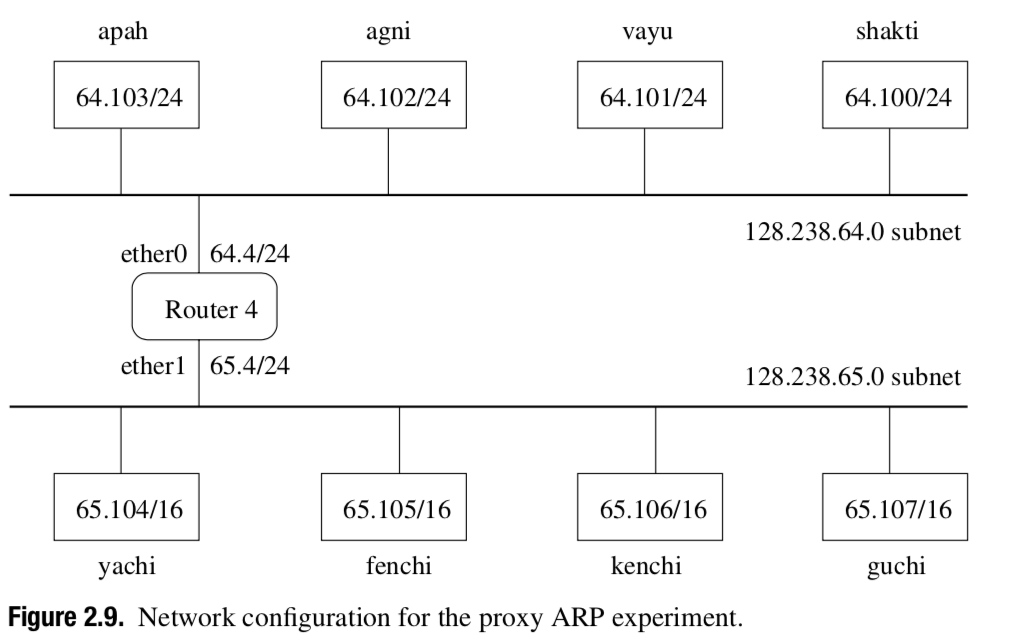
\includegraphics[width=0.7\textwidth]{img/figure2-9.png}
    \end{figure}
    
    \begin{report}
    \item Explain the operation of proxy ARP.

    \item Why can a host in the 128.238.65.0 subnet reach a host in the 128.238.64.0 subnet, even though they have different subnet IDs?

    \item What are the MAC addresses corresponding to hosts in the 128.238.64.0 subnet, in the ARP table of a host in the 128.238.65.0 subnet?

    \item Give one advantage and one disadvantage of using proxy ARP.
    \end{report}

\section{ARP Reboot Timeout}
    While \lstinline{tcpdump -ex -w exe7.out} (or run \lstinline{wireshark}) is running on all the hosts, reboot host \textit{h7}. 

    After \textit{h7} is started, terminate \lstinline{tcpdump} and run \lstinline{wireshark -r exe7.out &} to load the \lstinline{tcpdump} trace.
    Print the gratuitous ARP request for your lab report.
    
    \begin{report}
    \item What is the purpose of gratuitous ARP?

    \item List the sender IP address, target IP address, sender MAC address, and target MAC address of the gratuitous ARP you saved.
    \end{report}


\part{Exercise with ICMP and \texttt{ping}}
\section{ping ICMP}
    Use \lstinline[emph={remote-host}]{ping -sv remote-host} to test whether the remote host is reachable, while running:
    \lstinline[emph={your-host, remote-host}]{tcpdump -enx host your-host and remote-host}.
    Save the \lstinline{tcpdump} and \lstinline{ping} output for the future study on \lstinline{ping}.
    
    \begin{report}
    \item What ICMP messages are used by \lstinline{ping}?
    \end{report}

\section{ICMP Port Unreachable}
    While running \lstinline[emph={your-host, remote-host}]{tcpdump -x -s 70 host your-host and remote-host}, execute the following \lstinline{socket} command to send a UDP datagram to the remote host:
    \lstinline[emph={your-host, remote-host}]{socket -i -u -n1 -w1000 remote-host 88888}.

    Save the \lstinline{tcpdump} output for the lab report.

    \begin{report}
    \item Study the saved ICMP port unreachable error message (see Fig. 2.7).
    Why are the first 8 bytes of the original IP datagram payload included in the ICMP message?
    \end{report}

\section{\texttt{ping} ICMP}
    While \lstinline{tcpdump} is running to capture the ICMP messages, \lstinline{ping} a host with IP address 128.238.60.100. Save the \lstinline{ping} output.
    
    \begin{report}
    \item Can you see any traffic sent on the network? Why? Explain what happened from the \lstinline{ping} output.

    \item List the different ICMP messages you captured in Exercises 8, 9, and 10 (if any). Give the values of the type and code fields.
    \end{report}

\part{Exercises with IP address and subnet mask}
    In this section, we will observe what happens when the same IP address is assigned to two different hosts.
    We will also set an incorrect subnet mask for hosts and see what are the consequences.
    For the next two exercises, we split the current single segment network into two segments, Group A and Group B as shown in Table 2.3, so that they will not interfere with each other.

    \begin{table}[H]
        \caption{\textit{Table 2.3.} Host IP addresses and network masks for \textit{11 Duplicate IP}}
        \centering
        \begin{tabular}{ c c c c }
            \hline \hline
            Group & Host & IP Address & Subnet Mask \\
            \hline 
            Group A & h0 & 128.238.66.100 & 255.255.255.0 \\
                    & h1 & 128.238.66.100 & 255.255.255.0 \\
                    & h2 & 128.238.66.102 & 255.255.255.0 \\
                    & h3 & 128.238.66.103 & 255.255.255.0 \\
                    \hline
            Group B & h4 & 128.238.66.104 & 255.255.255.0 \\
                    & h5 & 128.238.66.104 & 255.255.255.0 \\
                    & h6 & 128.238.66.106 & 255.255.255.0 \\
                    & h7 & 128.238.66.107 & 255.255.255.0 \\
            \hline \hline
            \end{tabular}
    \end{table}

\section{Duplicate IP}
    Change the IP address of your workstation as shown in Table 2.3.

    Delete the entries for all hosts other than your own workstation from your workstation’s ARP table.

    Run \lstinline{tcpdump -enx} on all the hosts.
    Then, do the following three experiments.

    \begin{enumerate}
        \item Execute \lstinline{telnet} from one of two hosts with the duplicate IP address to a host with unique IP address (e.g.\ \textit{h0} –> \textit{h2} in Group A and \textit{h4} –> \textit{h6} in Group B).

        Now, from the other host with the duplicate IP address, execute \lstinline{telnet} command to the same host (\textit{h1} –> \textit{h2} or \textit{h5} –> \textit{h6}).

        Observe what happens and save the \lstinline{tcpdump} output and the ARP tables in all the hosts in your group.
        
        \item Execute \lstinline{telnet 128.238.66.100} (or \lstinline{telnet 128.238.66.104}) from \textit{h2} (or \textit{h6}).
        Which host provides the telnet connection?
        Why?
        
        \item Execute \lstinline{telnet 128.238.66.100} (or \lstinline{telnet 128.238.66.104}) from \textit{h3} (or \textit{h7}). Which host is connected to \textit{h3} (or \textit{h7})? Why?
    \end{enumerate}
    
    \begin{report}
    \item Explain what happened in the first case and why.
    Answer the questions for the second and third cases.
    \end{report}

\section{IP Subnets}
    Change the host IP addresses and the subnet masks as shown in Table 2.4. Since we still have two separate segments, Groups A and B can do the exercise independently.
    Note that two hosts in each group (\textit{h0} and \textit{h3} in Group A, or \textit{h4} and \textit{h7} in Group B) are assigned an incorrect subnet mask.

    Capture the packets with \lstinline{tcpdump -e} for the following cases.

    \begin{enumerate}
        \item When \textit{h0} (\textit{h4}) \lstinline{ping}s one of the hosts that have the correct subnet mask.
        
        \item When \textit{h3} (\textit{h7}) \lstinline{ping}s one of the hosts that have the correct subnet mask.

        Now, copy the output displayed from the \lstinline{ping} window in \textit{h3} (\textit{h7}).
        Share the saved output message with other students.
        
        \item When a host with the correct subnet mask \lstinline{ping}s \textit{h0} (\textit{h4}).
        
        \item When a host with the correct subnet mask \lstinline{ping}s \textit{h3} (\textit{h7}).
    \end{enumerate}
    
    To avoid confusion, only one machine in each group should generate traffic in each case.
    Clearly, this exercise has to be performed as a team.
    \begin{table}[H]
        \caption{\textit{Table 2.4.} Host IP addresses and network masks for \textit{12 IP subnet}}
        \centering
        \begin{tabular}{ c c c c }
            \hline \hline
            Group & Host & IP Address & Subnet Mask \\
            \hline 
            Group A & h0 & 128.238.66.100 & 255.255.255.240 \\
                    & h1 & 128.238.66.101 & 255.255.255.0~~~ \\
                    & h2 & 128.238.66.102 & 255.255.255.0~~~ \\
                    & h3 & 128.238.66.120 & 255.255.255.240 \\
                    \hline
            Group B & h4 & 128.238.66.104 & 255.255.255.240 \\
                    & h5 & 128.238.66.105 & 255.255.255.0~~~ \\
                    & h6 & 128.238.66.106 & 255.255.255.0~~~ \\
                    & h7 & 128.238.66.121 & 255.255.255.240 \\
            \hline \hline
            \end{tabular}
    \end{table}
    
    \begin{report}
    \item Explain what happened in each case according to the \lstinline{tcpdump} outputs saved.
    Explain why \textit{h3} (or \textit{h7} in Group B) could not be reached from other hosts, whereas \textit{h0} (or \textit{h4} in Group B), which has the same incorrect subnet mask, could communicate with the other hosts.
    \end{report}
\end{document}
